\section{Limitations of LLMs}
\label{sec:llm_discussion}

With our findings from the human study in mind, we now turn to LLM performance to provide insights that could inform future methods for improving idea generation systems. 
Our ideation agent is motivated by two potential strengths of LLMs: their ability to scale by generating a vast number of ideas - far more than any human could - and the possibility of filtering these ideas to extract the best ones from the large pool. 
In theory, this approach could lead to high-quality ideas by leveraging inference scaling. However, we present empirical evidence that this naive assumption about scaling idea generation has significant limitations.

% This section offers some insights from an LLM perspective on idea generation to help future research further improve their LLMs. 
% On a very high level, we hope LLMs can generate a large number of diverse ideas, automatically evaluate these ideas, and finally select the best ideas out of all the generations. 
% In this way, we can get more high-quality ideas by scaling up inference. 
% However, we show empirical evidence that current LLMs are not capable enough for this paradigm. 



\subsection{LLMs Lack Diversity in Idea Generation}
\label{sec:duplication}


\begin{figure}[t]
\small
\centering
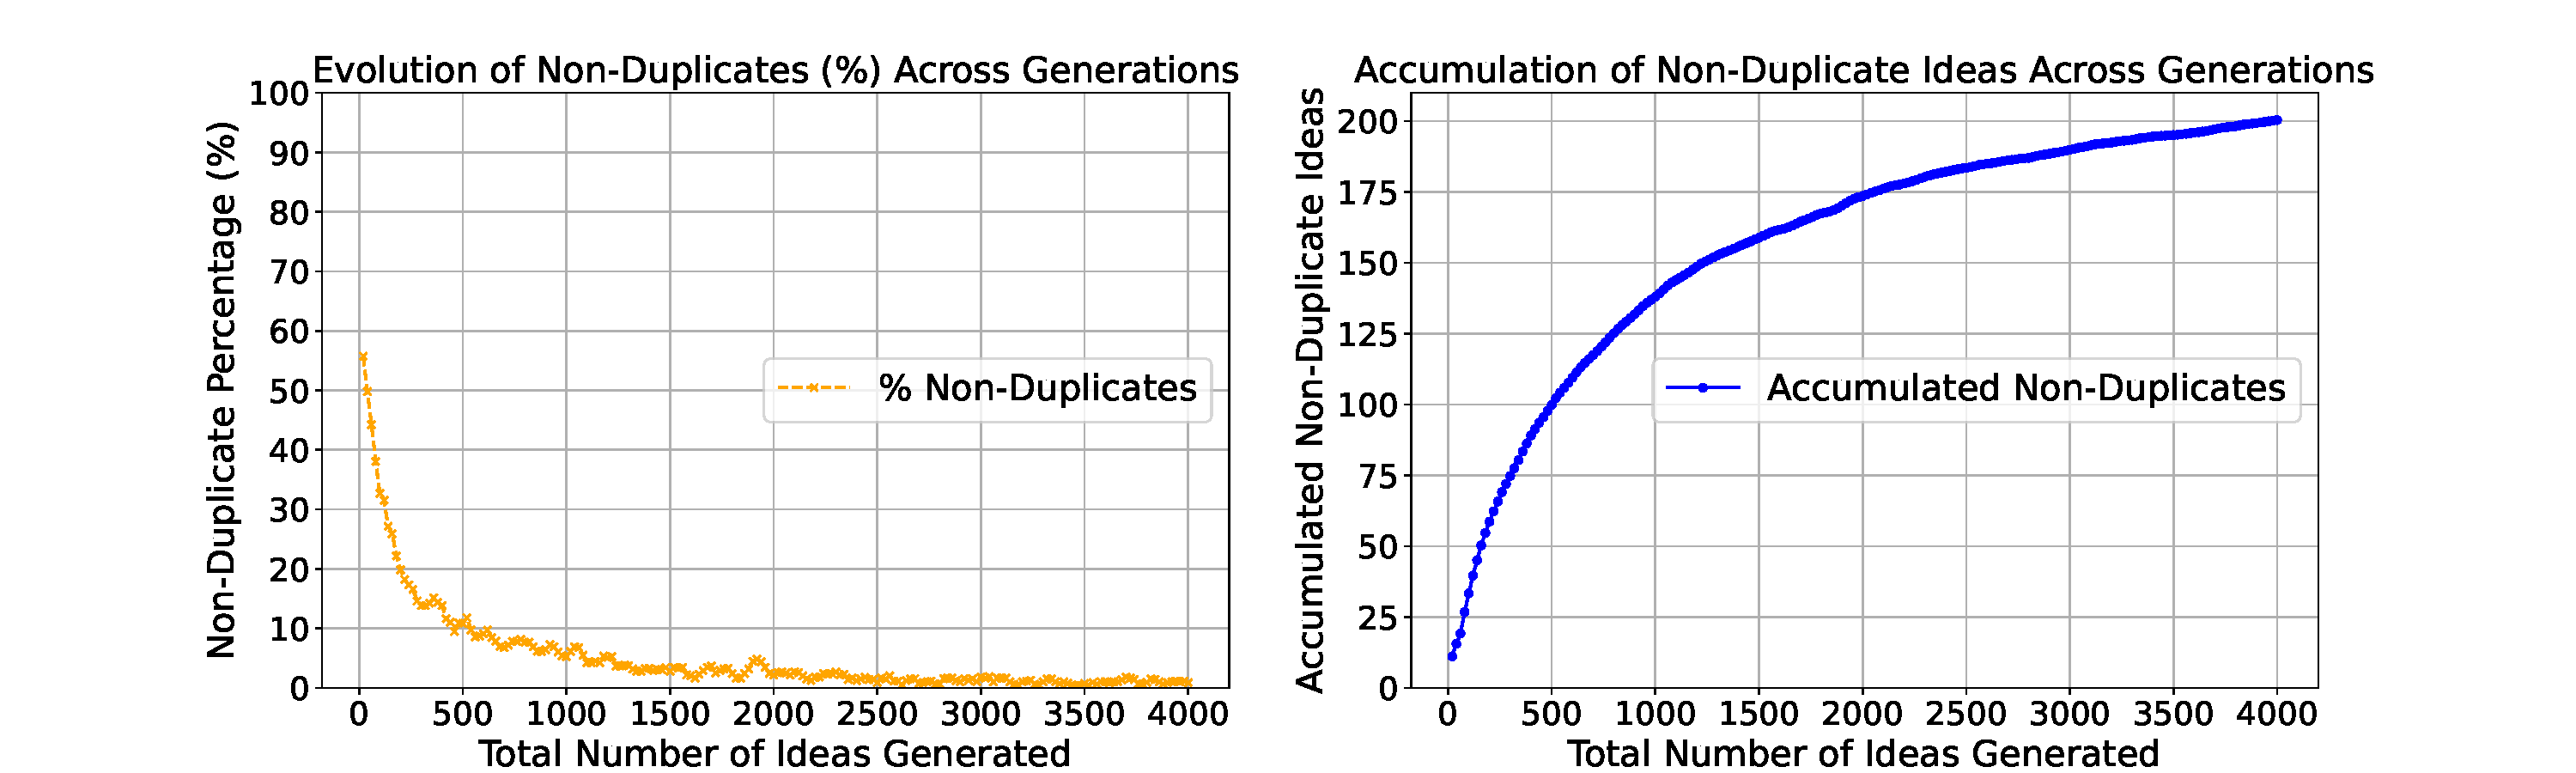
\includegraphics[width=\textwidth]{figures/duplication_comparison.pdf}
\caption{Measuring duplication of AI-generated ideas: the left figure plots the percentage of non-duplicate ideas in each new bucket of generated ideas; the right figure plots the accumulated non-duplicate ideas as the agent keeps generating new ideas. All data points are averaged across all topics.}
\label{fig:duplication}
\end{figure}


We adopted an over-generate and rank paradigm in idea generation. This raises the question: is there an upper limit to how many new ideas LLMs can generate? To answer this question, we take a closer look at 4000 generated seed ideas for each topic. 


We encode all raw ideas with \texttt{all-MiniLM-L6-v2} from Sentence-Transformers. For each idea, we compute its cosine similarity with all previously generated ideas on the same topic. 
We consider an idea as a duplicate if it has a similarity of above 0.8 with any of the previously generated ideas. 
In Figure~\ref{fig:duplication}, we show that as the agent keeps generating new batches of ideas, the percentage of non-duplicates in newly generated batches keeps decreasing, and the accumulated non-duplicate ideas eventually plateau. In fact, out of the 4000 generated seed ideas, there are only 200 non-duplicate unique ideas. 
This sets a bottleneck on our inference-time scaling since increasing the number of generated ideas simply leads to repeating duplicate ideas. 

% \newpage

\subsection{LLMs Cannot Evaluate Ideas Reliably}
\label{sec:self_eval}


\begin{wraptable}{r}{0.34\textwidth}
\centering
\small 
\begin{tabular}{l c} 
 \hline
 & Consistency \\ 
 \hline
 Random & 50.0 \\
 NeurIPS'21 & 66.0 \\
 ICLR'24 & 71.9 \\ 
 Ours & 56.1 \\
 \hline
 GPT-4o Direct & 50.0 \\ 
 GPT-4o Pairwise & 45.0 \\
 Claude-3.5 Direct & 51.7 \\ 
 Claude-3.5 Pairwise & 53.3 \\ 
 ``AI Scientist'' Reviewer & 43.3 \\
 \hline 
\end{tabular}
\caption{Review score consistency among human reviewers (first block) and between humans and AI (second block).}
\label{table:agreement}
\end{wraptable}

Most prior works have adopted \emph{LLM-as-a-judge} for evaluating research ideas~\cite{AIScientist} motivated by the observation that LLMs can have a higher agreement with human evaluators than the inter-human agreement. However, we offer some empirical evidence that LLMs cannot evaluate ideas reliably yet. 

Concretely, we use the average review score of each idea to rank the top and bottom $25\%$ of all our collected human and AI ideas, 
and use this to benchmark various LLM evaluators. Specifically, we obtain the LLM predicted scores of all ideas and set the median score as the threshold to measure their accuracy on our balanced idea ranking data. 

In the second block of Table~\ref{table:agreement}, we compare several different LLM evaluators: 1) directly giving the review criteria and prompting for a final score~\cite{Yang2023LargeLM,Li2024MLRCopilotAM,Baek2024ResearchAgentIR}; 2) our pairwise ranker as described in Section~\ref{sec:agent_ranking}; and 3) the ``AI Scientist'' reviewer agent~\cite{AIScientist}. All of these LLM evaluators \textbf{have a lower agreement than our expert reviewers' scores}. Even the best LLM evaluator --- our own Claude-3.5 pairwise ranker --- only achieves an accuracy of 53.3\%, lower than our inter-reviewer consistency of 56.1\%. 

Even if AI-human agreement eventually matches or exceeds human-human agreement, simply meeting this baseline does not imply that AI-as-a-reviewer is meaningful, since we may be trading variance for bias, where AI reviewers are more consistent but rely on spurious correlations~\cite{Durmus2022SpuriousCI}. Our findings in Table~\ref{table:agreement} are consistent with these brittleness concerns, as we find a significant drop in AI-human agreement scores under our study compared to the original studies.
%Moreover, AI reviewers suffer from other major weaknesses such as high sensitivity and brittleness. They may work well on the validation sets the creators optimize them for, yet fail outside the training condition, as suggested by the difference between the ``AI Scientist'' Reviewer's in-distribution accuracy ($65.0\%$ reported in~\citet{AIScientist}) and out-of-distribution accuracy ($43.3\%$ in our Table~\ref{table:agreement}).  

Finally, even though Claude-3.5 pairwise agreements may seem close to human agreement, many other pieces of evidence throughout the paper leads us to be cautious about the use of LLM-as-a-judge in such a complex and subjective task. These include our findings on the significant discrepancy between the agent's top-ranked ideas and the human expert's top-ranked ideas (Appendix~\ref{sec:overlap}) and how the \texttt{AI Ideas + Human Rerank} condition tends to score higher than the \texttt{AI Ideas} condition on all metrics in Section~\ref{sec:results}. 
These limitations of LLM auto-evaluation not only constrain the effectiveness of our over-generate-and-rank paradigm for idea generation but also raise concerns about trusting conclusions that are based primarily on LLM evaluators.

% Throughout the paper, we showed multiple evidences that the automatic ranking of ideas by the LLM agent is not reliable yet. For example, Appendix~\ref{sec:overlap} shows that there is a significant discrepancy between the agent's top-ranked ideas and the human expert's top-ranked ideas. 
% And in Section~\ref{sec:results} we observe that the \texttt{AI Ideas + Human Rerank} condition significantly scores higher than the \texttt{Human Ideas} conditions on excitement across all tests while the \texttt{AI Ideas} condition does not. 
% Moreover, the benchmarking result of our LLM ranker is only 71.4\% accuracy on the much simplified binary task of deciding which paper is accepted by ICLR out of random pairs of accepted and rejected papers. 
% These results suggest that LLMs are far from perfect in ranking ideas. 
% This not only constrains the effectiveness of our over-generate-and-rank paradigm of idea generation but also casts doubts on recent attempts to rely entirely on LLMs for evaluating generated ideas~\cite{AIScientist}. 